\chapter{Обзор литературы} \label{chapt1}

\section{Современное состояние исследований оптических частотных гребенок и солитонов в микрорезонаторах} \label{sect1_1}

Открытие и развитие оптических частотных гребенок на основе фемтосекундных лазеров с синхронизацией мод оказало огромное влияние на науку и технологии с момента их первоначальной демонстрации в 2000 году \cite{Jones635,PhysRevLett.84.5102}. Это открытие было отмечено Нобелевской премией по физике в 2005 г \cite{Hall2006}. Помимо приложений в прецизионной частотной метрологии и для создания атомных часов \cite{Diddams2001,Udem2002,Ye2005,Diddams2004}, возможность эффективного контроля амплитуды и фазы точно определенных спектральных линий открыла новые подходы для генерации аттосекундных импульсов, спектроскопии веществ \cite{Stowe2008,Diddams2007,Ideguchi2013,Holzwarth2000}, обработки оптических сигналов и радиофотоники \cite{Gao2006,Torres2014}, калибровки астрономических эшелле-спектрографов \cite{Steinmetz2008} и синтеза спектрально чистых СВЧ сигналов \cite{Fortier2011}.

Открытые в лаборатории профессора Т. Киппенберга в 2007 году оптические частотные гребенки в микротороидах из плавленого кварца \cite{DelHaye2007} вызвали новую волну интереса и исследований в области микрорезонаторов и частотной метрологии \cite{Kippenberg2011}. Оптическая частотная гребенка в микрорезонаторе представляет собой набор эквидистантных спектральных линий, получающихся каскадно при накачке высокодобротной моды пассивного микрорезонатора из материала с кубичной нелинейностью с помощью мощного, узкополосного и перестраиваемого лазера непрерывной мощности. Керровские частотные гребенки имеют расстояния между линиями 5-1000 ГГц и позволяют достичь уровня минитюаризации и энергоэффективности устройств, трудно достижимого для гребенок, полученных с помощью фемтосекундных лазеров с синхронизации мод. Над развитием этой новой области работают около 10 экспериментальных групп и еще несколько теоретических групп. За 11 прошедших с открытия лет был проведен обширный теоретический анализ и численное моделирование богатой нелинейной динамики процесса формирования оптических гребенок, были проведены эксперименты, демонстрирующие их фундаментальные свойства и важнейшие практически применения. Количество публикаций с 2014 по 2018 годы с ключевыми словам солитоны в оптических резонаторах составило около 600, из них несколько десятков в самых высокорейтинговых научных журналах. В случае преодоления нескольких нерешенных проблем, оптические частотные гребенки из микрорезонаторов могут стать востребованным коммерческим продуктом.

В отличие от частотных гребенок, получаемых при синхронизации мод фемтосекундного лазера, произвольные оптические частотные гребенки из микрорезонатора не представляют собой короткие импульсы во временном представлении из-за произвольных фазовых соотношений между отдельными спектральными линиями, появляющимися в процессе каскадного формирования гребенки \cite{Herr2012,Chembo2010}. Некогерентные шумные оптические гребенки были продемонстрированы в различных структурах, в том числе в кристаллических резонаторах из различных фторидов при накачке в ближнем ИК \cite{Savchenkov2008,Grudinin2012,Liang2011,Grudinin2009,Henriet:15}, в том числе шириной в октаву \cite{DelHaye2011}, в интегральных микрорезонаторах из нитрида кремния ($Si_3N_4$) \cite{Levy2010,Okawachi2011,Johnson2012,Huang2015}, в планарных системах, изготовленных из стекла Hydex \cite{Moss2013,Razzari2010}, а также в других диэлектрических материалах: нитриде алюминия $AlN$ \cite{Jung2013}, фосфиде галлия $GaP$ \cite{2018arXiv180803554W} и алмазе \cite{Hausmann2014}. Важным типом резонаторов являются кольцевые волоконные резонаторы ($SiO_2$), в которых динамика гребенок описывается теми же уравнениями, и возможно прямое измерение профиля поля внутри резонатора благодаря длительности импульса $5-10$ пс. Именно в волоконных кольцевых резонаторах было впервые продемонстрировано формирование и распространение солитонов, но при накачке затравочным импульсом \cite{Leo2010}.

Большим прорывом стало теоретическое предсказание и экспериментальная демонстрация высококогерентных частотных гребенок, линии которых синхронизированы по фазе \cite{Herr2014}. Такая малошумная оптическая гребенка соответствует оптическому временному солитону, распространяющемся внутри микрорезонатора. Для стационарного режима распространения солитонов необходим баланс между дисперсией групповой скорости и нелинейностью в микрорезонаторе, а также между потерями и накачкой через параметрическое преобразование частоты. Предложенный метод основан на перестройке частоты лазера накачки из области синей отстройки от моды микрорезонатора в красную сторону, в область существования солитона. Этот метод позволил генерировать когерентные и широкополосные оптические гребенки, которые могут быть достигнуты повторимо. Эта работа показала возможность генерации фемтосекундных оптических импульсов с малым джиттером из вакуумных флуктуаций мод микрорезонатора. C помощью этого метода оптические солитоны были получены в кристаллических цилиндрических \cite{Herr2014} и кварцевых микротороидах \cite{Yi2015} при накачке на длине волны около $1550$ нм. В этих же двух работах было произведено частотно-разрешенное оптическое стробирование (FROG) для экспериментального подтверждения импульсного временного профиля электрического поля в микрорезонаторе. В работе \cite{Brasch2016} впервые показали формирование оптического солитона и генерацию высоко когерентной гребенки спектральной шириной в $2/3$ октавы в $Si_3N_4$ кольцевом микрорезонаторе, интегрированном на чип. Также солитонная гребенка была продемонстрирована в интегральном кольцевом резонаторе из кремния $Si$ при накачке в среднем ИК диапазоне, где двухфотонное поглощение в материале мало \cite{Yu2016}, настройка на солитонный режим достигался путем инжекции свободных носителей в PIN структуру и мониторинга тока на ней. Недавняя работа показала возможность генерации оптических солитонов в интегральном резонаторе из ниобата лития $LiNbO_3$ \cite{2018arXiv181209610H}, где квадратичная нелинейность не равна нулю, так что одновременно с солитонной гребенкой с центром на 1550 нм образовывалась гребенка на удвоенной частоте 775 нм. Таким образом по состоянию на конец 2018 г. солитонный режим оптических гребенок был продемонстрирован в меньшем количестве материалов ($MgF_2, Si_3N_4, Si, SiO_2, LiNbO_3$), чем шумная оптическая гребенка.

В последние годы было продемонстрировано несколько методов, позволяющих обойтись без быстрой перестройки частоты лазера накачки для генерации солитонного режима: один из них базируется на использовании фазово модулированной накачки \cite{Jang2015ol}, второй на тепловых эффектах с использованием дополнительного нагревательного элемента \cite{Joshi2016}. При нагреве микрорезонатора происходит сдвиг резонансных частот микрорезонатора относительно частоты лазера накачки, что эквивалентно ранее описанному процессу перестройки частоты лазера накачки. Была показана возможность детерминированного получения односолитонного режима с гладкой огибающей спектра, важного для практических применений, например, в спектроскопии с помощью двух гребенок. Это осуществлялось либо контролируемым нагревом и охлаждением нагревательного элемента для резонатора \cite{Joshi2016}, либо обратной медленной перестройкой частоты лазера накачки \cite{Karpov2017}.

Было опубликовано множество работ, посвященных численному моделированию динамики генерации солитонов \cite{Lamont2013,Hansson2016}, анализу устойчивости решений \cite{Godey2014}, детерминированной генерации состояний с заданным числом солитонов \cite{Jaramillo2015}, численному предсказанию бризерных режимов \cite{Matsko2012}, эффективности нелинейного преобразования мощности накачки в линии солитонной гребенки \cite{Bao2014}. Экспериментально были продемонстрированы состояния оптических гребенок, где все линии находились в постоянных фазовых соотношениях, но динамика такой синхронизации была отличной от формирования солитонов \cite{Saha2013,DelHaye2014}. Экспериментально были продемонстрированы "солитонные кристаллы" - состояния, при которых в микрорезонаторе распространяется максимально возможное количество солитонов, эти состояния имеют сложный спектр и другую тепловую динамику генерации \cite{Cole2017crystals}. Эксперименты с оптическом пинцетом во временном представлении для "записывания и удаления" солитонов из последовательности в волоконном кольцевом резонаторе \cite{Jang2015}. Численно исследовалось влияние дисперсии высоких порядков \cite{Wang2014} на свойства солитонов. В работе \cite{HerrPRL2014} описаны механизмы, препятствующие образованию солитонов в микрорезонаторах: большая по модулю дисперсия групповой скорости и эффекты нормального расщепления мод вблизи моды накачки.

В работе \cite{Jost2015} продемонстрирована солитонная гребенка из микрорезонатора и привязка лазера накачки к стабилизированной гребенке из фемтосекундного лазера, тем самым достигается полностью стабилизированная оптическая гребенка из кристаллического микрорезонатора. В последующей работе \cite{Jost:15} была продемонстрирована привязка солитона из кристаллического микрорезонатора на себя с использованием сильно нелинейного волокна для уширения спектра солитона до октавы. Таким способом были когерентно привязаны оптическая частота лазера накачки 190 ТГц и СВЧ частота повторения солитона 14 ГГц. Позже в работе \cite{Brasch2017} была продемонстрирована привязанная на себя гребенка, получаемая из солитона на $Si_3N_4$ чипе, без внешнего уширения спектра, а с использованием техники 2f-3f, когда удвоенная частота синего края спектра гребенки была близка к утроенное частоте красного края спектра, и результирующий сигнал биений стабилизировался.

Отдельно необходимо выделить работу \cite{Obrzud2017}, в которой впервые продемонстрирован оптический солитон в компактном микрорезонаторе при накачке не лазером непрерывной мощности, а оптическим импульсом, совпадающим по частоте повторения с межмодовым расстоянием микрорезонатора. Микрорезонатором служил высокодобротный одномодовый резонатор Фабри-Перо, выполненный из куска обычного оптоволокна SMF, с напылением по торцам. Наблюдалось возникновение фемтосекундных солитонных импульсов поверх резонансно-усиленных импульсов накачки. При этом солитон был привязан к накачивающим импульсам, что позволяло контролировать частоту его повторения и отстройку фазы несущий от максимума огибающей солитона.

Ширина полосы параметрического усиления ограничена только окном прозрачности материала микрорезонатора, что потенциально позволяет генерировать гребенки от видимого до среднего ИК диапазонах при достижении аномальной дисперсии групповой скорости в резонаторе и наличии достаточно мощного лазера накачки на заданной длине волны. Одной из приоритетных задач является расширение спектрального покрытия существующих керровских частотных гребенок. Были продемонстрированы когерентные солитонные гребенки в ближнем ИК диапазоне в микротороидах из плавленного кварца с добротностью $8*10^7$ \cite{Lee2017} и интегральном $Si_3N_4$ микрокольце с оптимизированной дисперсией \cite{Karpov2018} при накачке лазером на длине волны 1 мкм. Синий край спектра достигал значений $776$ нм.

При накачке лазером на длине волны 1.55 мкм (телекомуникационный С-диапазон) и 1.3 мкм (О-диапазон) интегральных резонаторов из $Si_3N_4$ были получены оптические солитоны, спектр которых перекрывает октаву \cite{Li:17,Pfeiffer:17}. Оптимизируя процесс фабрикации резонатора с областью свободной дисперсии (ОСД) 1 ТГц, была достигнута гребенка шириной в октаву, т.ч. по краям спектра наблюдались более интенсивные дисперсионные волны на тех частотах, где дисперсия меняла знак благодаря специально подобранному дизайну сечения резонатора. Максимальная ширина гребенки составила 200 ТГц при мощности накачки в волноводе всего около 100 мВт.

Другим направлением исследований является генерация керровских частотных гребенок в среднем ИК диапазоне. Этот диапазон интересен тем, что в нем находятся колебательные уровни многих органических молекул, из-за чего его называют диапазоном “молекулярной дактилоскопии” \cite{Diddams2007,Schliesser2012}. Средний ИК изучается в основном с помощью инфракрасных-Фурье спектрометров \cite{Griffiths2006}. Технология генерации керровских гребенок в среднем ИК остается сравнительно слаборазвитой, особенно в сравнении с оптическими частотными гребенками из квантово-каскадных лазеров на чипе \cite{Hugi2012}. Количество публикаций, посвященных этой проблеме, сравнительно мало. При использовании параметрического лазера непрерывного излучения в качестве накачки была показана возможность генерации оптических гребенок в среднем ИК на длине волны 2.5 мкм в кристаллическом микрорезонаторе\cite{Wang2013}, ширина гребенки составила 200 нм, с расстоянием между линиями около 100 ГГц. Также генерация гребенки со спектральной шириной, превышающей половину октавы, была продемонстрирована в микрорезонаторах из $CaF_2$ и $MgF_2$ при накачке квантово-каскадным лазером на длине волны 4.3 мкм \cite{Savchenkov2015}. Этот результат не был воспроизведен в других группах, т.к. фурье спектрометры на данный диапазон имеют низкий динамический диапазон и плохое разрешение (более 10 ГГц). Любая малая амплитудная флуктуация лазера накачки отображается как набор спектральных компонент. Также было показано \cite{Lecaplain2016}, что $MgF_2$ имеет добротность не более $10^7$ на длине волны 4.5 мкм, что недостаточно для генерации гребенки при имеющейся мощности квантово-каскадного лазера (QCL). Самые лучшие результаты были достигнуты в интегральных структурах из кремния (микрокольца), выполненных по CMOS совместимой технологии. При накачке на длине волны 2.6 мкм мощностью 1.2 Вт была достигнуты шумная гребенка шириной от 2100 до 3500 нм, с расстоянием между линиями в 100 ГГц \cite{Griffith2015}. В работе \cite{Griffith2016} при накачке на длине волны 3 мкм продемонстрирована генерация гребенки шириной 2.4-4.3 мкм. Большим преимуществом в работе было использование PIN структуры на кремниевом волноводе одновременно для контроля динамики гребенки через контроль времени жизни свободных носителей и для детектирования индуцированного тока трехфотонного поглощения. Измеряя спектр сигнала на таком интегрированном PIN диоде был сделан вывод о состоянии гребенки с малыми фазовыми шумами. В качестве материала, пригодного для генерации частотных гребенок в среднем ИК, изучались фториды бария, стронция и кальция, различные ZBLAN стекла \cite{Grudinin2016,Way2012,Lecaplain2016}.

Еще одним важным направлением исследований является возможность генерации когерентных гребенок в режиме нормальной дисперсии групповой скорости \cite{Xue2016nano}, т.к. материальная дисперсия большинства исследуемых материалов в видимом и ближнем ИК диапазоне длин волн является нормальной. В видимом диапазоне керровские частотные гребенки с большим межмодовым расстоянием (>10 ГГц) могут, в частности, использоваться для калибровки эшелле спектрографов \cite{Benedick2010,Glenday2015} и приложений рамановской спектральной визуализации. Видимый диапазон привлекателен тем, что в нем возможна детектирование биологических веществ \cite{Karpov2018} из-за наличия в нем окна спектра пропускания воды, и он характеризуется большими сечениями комбинационного рассеяния. В основном до настоящего времени для генерации частотных гребенок в видимом диапазоне использовалось совместное действие квадратичной и кубичной нелинейностей в кристаллических или интегральных микрорезонаторах \cite{Miller2014,Jung2014}.

Из-за наличия пиков поглощения в УФ многие диэлектрические материалы имеют нормальную дисперсию групповых скоростей в видимом диапазоне и ближнем ИК, что препятствует генерации светлых солитонов. Теоретически и экспериментально узкие керровские частотные гребенки при нормальной ДГС изучались в кристаллических микрорезонаторах \cite{Coillet2013,Liang2014,Henriet2015} и микрокольцах на чипе \cite{Huang2015prl,Xue2015}, было сделано утверждение о достижении низкого уровня фазового шума оптических линий. Также было теоретически и экспериментально продемонстрировано существование темных временных импульсов \cite{Godey2014,ParraRivas2016}. В работе \cite{ParraRivas2016} существование темных солитонов было связано с наличием волн переключения между двумя решениями постоянной величины. Было показано, что в системе с двумя связанными микрорезонаторами можно управлять динамикой генерации темных импульсов через контроль связи между резонаторами \cite{Liu2015}. В работе \cite{PhysRevLett.121.257401} экспериментально продемонстрированы бризерный режимы темных импульсов. Однако на сегодняшний день полное понимание динамики, в том числе механизмов, обеспечивающих генерацию керровских частотных гребенок с малым шумом в режиме нормальной дисперсии, отсутствует.

Еще одним направлением исследований в области микрорезонаторных частотных гребенок является разработка методов увеличения их ширины. Одним из исследуемых в последнее время способов является взаимодействие временных солитонов и дисперсионных волн, иногда по аналогии с классическим эффектом Черенкова называемых индуцированным  солитонами черенковским излучением \cite{Akhmediev1995,Barashenkov2011,Milian2014}. При накачке микрорезонатора в области аномальной дисперсии возможна генерация светлого солитона. Если его длительность достаточно мала, то его спектр распространяется в область нормальной дисперсии и солитон может генерировать дисперсионную волну – пик излучения вблизи точки нулевой дисперсии. Формирование дисперсионной волны в присутствии солитона может способствовать уширению полосы генерации гребенки в область нормальной дисперсии без потери когерентности \cite{Brasch2016,Jang2014,Pfeiffer:17}. Дисперсионные волны возникают и при наличии сильных эффектов нормального расщепления мод (взаимодействие различных пространственных семейств мод микрорезонатора) \cite{Yang2016,Matsko:16}. Показано, что самовоздействие солитона, может сдвигать частоту дисперсионной волны.

Для генерации и реализации эффективного взаимодействия солитонов и дисперсионных волн должны выполняться определенные дисперсионные соотношения, поэтому разрабатывается множество методов получения оптимальной дисперсии (dispersion engineering). Дисперсия резонатора может быть специально задана с помощью подбора размеров сечения планарного кольца \cite{Okawachi2014,Pfeiffer:17}, или с помощью микроструктурирования его формы при точении кристаллов \cite{Grudinin2012,Grudinin2015,Nakagawa2016}. Теоретически показана возможность достижения аномальной дисперсии в октавном диапазоне для резонаторов с ОСД меньше 100 ГГц, что позволит напрямую измерить частоту повторения светлого солитона с помощью современной СВЧ электроники.

Совершенно новым динамическим методом управления дисперсией групповой скорости интегрального микрорезонатора стало покрытие его графеном. Так в работе \cite{Yao2018}, на сектор интегрального микрокольца из $Si_3N_4$ был нанесен йонный гель и монослой графена, управляя напряжением на затворе получившегося транзистора, можно управлять хроматической дисперсией микрорезонатора, изменяя Ферми уровень графена в пределах 0.45-0.65 эВ при усилении с помощью йонного транспорта и тепловых эффектов в йонном геле. При напряжениях в диапазоне от 0 до -2 В линейное поглощение в графене на длине волны 1600 нм мало из-за блокады Паули. Добротность структуры сохранялась на уровне $1\times10^6$ Было экспериментально измерено изменение дисперсии второго (от -62 фс$^2$ мм$^{-1}$ до +9 фс$^2$ мм$^{-1}$), изменение эффективного показателя преломления микрорезонатора в зависимости от приложенного напряжения на затворе. Были продемонстрированы режимы генерации модуляционной неустойчивости, шумной гребенки с дисперсионной волной, многосолитонный режим, солитонные кристаллы при изменении напряжения на затворе. Также для режима модуляционной неустойчивости была показана модуляция амплитуды оптических линий с частотой до 60 кГц с помощью модуляции напряжения на затворе.

Большой интерес вызывает возможность использования эффектов рамановского и бриллюэновского рассеяния для генерации частотных гребенок и контроля их свойств. Активно исследуется влияние рамановского рассеяния на генерацию и свойства диссипативных солитонов в оптических микрорезонаторах: эффект сдвига спектрально максимума солитона, Raman induced soliton self-frequency shift \cite{Hansson2014ol,Milian2015,Yi2016,Karpov2016,Bao2017}. Также в работах \cite{Chembo2015,Chembo2016} исследовалась возможность генерации оптической частотной гребенки в полосе рамановского рассеяния в области нормальной дисперсии групповой скорости. В работе \cite{Chembo2015} экспериментально была продемонстрирована генерация оптической частотной гребенки в кристаллическом резонаторе из $MgF_2$ при накачке на 1064 нм в присутствии интенсивного спектрального максимума, вызванного вынужденным комбинационным рассеянием.

Уникальным результатом стала демонстрация впервые в оптических системах Стоксовских солитонов, при накачке микротороида из плавленого кварца $SiO_2$ на длине волне 1550 нм, и одновременно индуцированного им солитона в области рамановского пика на 1650 нм \cite{Yang2016stokes}. Солитоны были образованы на разных поперечных модах микрорезонатора, и достигались благодаря оптимизации условий Рамановского взаимодействия во времени и пространстве.

Отдельно отметим работы, в которых изучались бризерные режимы солитонов \cite{Matsko2012}, в кристаллах \cite{Lucas2017breather}, в интегральных резонаторах \cite{PhysRevLett.117.163901,Yu2017breather}, как при аномальной \cite{Yu2017breather}, так и нормальной дисперсиях микрорезонатора \cite{PhysRevLett.121.257401}. Хотя во всех численных моделированиях бризерный режим легко получается, и были приведены убедительные экспериментальные измерения амплитуды и периода бризеров, детальная достоверная классификация и теоретическое описание этих сложных режимов для микрорезонаторов сделаны не были.

Наблюдение диссипативных керровских солитонов в микрорезонаторах вызвало не только интерес к изучению богатой нелинейной физики солитонов, но и демонстрации множества применений в высокоточной метрологии и других технологиях. Перечислим основные экспериментально продемонстрированные применения.

Важным лабораторным применением могут быть оптические часы. Экспериментальная демонстрация таких часов дана в \cite{Papp2014}. Модулированный по амплитуде лазер с максимальной мощностью $140$ мВт возбуждает микродиск из плавленого кварца. Генерируется гребенка, покрывающая $20$ нм интервал около накачки на $1560$ нм. Межмодовое расстояние составило $33$ ГГц. Далее гребенка расширяется до $200$ нм при ее пропускании через сильно нелинейное волокно. Новый спектр покрывает частоту рубидиевого стандарта (после удвоения частоты). Выбираются две линии гребенки на расстояний 108 мод друг от друга ($1560$ и $1590$ нм соответственно), которые привязываются через дополнительные лазеры к рубидиевым переходам. Выходным сигналом часов является разность частот между линиями гребенки. Она составила $33$ ГГц. Стабильность выходного сигнала лучше, чем у рубидиевого перехода в 108 раз. Девиация Аллана достигала $5\times10^{-12}$ при измерении за $10^4$ сек.

Солитонные оптические гребенки были использованы для калибровки астрономических эшелле-спектрографов в телекоммуникационном С-диапазоне \cite{Obrzud2019,Suh2019}. Этими группами независимо были предприняты попытки детектирования периодических Допплеровских спектральных сдвигов известных экзопланет на телескопах на Канарских островах и Гавайях. Для обнаружения экзопланет с длинным периодом требуется точность измерения радиальной скорости менее 10 см/c на временах порядка годов. В работе \cite{Suh2019} использовался кварцевый микротороид, несущая солитона был привязана к линии поглощения цианида водорода, а частота повторения после деления к рубидиевому стандарту. Расстояние между линиями составило 22 ГГц, что очень удобно для калибровки спектрографов в отличие от гребенок из фемтосекундных лазеров с типичным межмодовым расстоянием в сотни МГц. В статье \cite{Obrzud2019} использовался солитон из интегрального кольца из нитрида кремния, привязанный по несущей к стабилизированной гребенке из фемтосекундного лазера. Была достигнута точность калибровки эквивалентная радиальной скорости в 25 см/c, что существенно лучше, чем при калибровке катодной лампой. Однако, никакого измерения спектрального сдвига известных экзопланет в статьях не дано, причиной указана нестабильность самого спектрографа.

Солитонные оптические гребенки были успешно применены в прямой спектроскопии поглощения веществ с использованием двух гребенок, слабо отличающихся по межмодовому расстоянию (dual comb spectroscopy) в ближнем \cite{Suh2016} и среднем ИК диапазоне\cite{Yu2018}. В этом методе сбиваются два одинаковых источника оптических частотных гребенок в ближнем или среднем ИК с немного различными частотами повторения, и генерируется сигнал биений на фотодетекторе в форме гребенки, но уже в радио диапазоне частот, что может быть использовано для восстановления профилей поглощения веществ в быстром, компактном устройстве без подвижных механических частей. Оптическое разрешение определяется межмодовым расстоянием гребенок, а скорость определяется разностью между частотами повторений. Одна гребенка используется как локальный осциллятор, другая используются для получения оптической спектральной картины исследуемого образца. Результирующие биения двух гребенок дают радиочастотный сигнал, содержащий информацию о линиях поглощения. Первая демонстрация спектроскопии с использованием двух солитонных гребенок из двух отдельных микрорезонаторов из плавленного кварца была дана в \cite{Suh2016}, оптические гребенки шириной 4 ТГц с центром на 1.5 мкм были перенесены в радиодиапазон, проведена спектроскопия произвольного сигнала вейвшейпера (оптического генератора сигнала произвольной формы) и линий поглощения ячейки с $HCN$. В работе \cite{Yu:17} была продемонстрирована сканирующая оптическая спектроскопия при одновременном сканировании по частоте всех линий одной гребенки. В работе \cite{2018arXiv181209789S} была продемонстрирована прямая спектроскопия атомного перехода в рубидии с помощью оптической гребенки, а также стабилизация всех линий гребенки на этот переход, т.ч. флуктуации абсолютной частоты каждой линии составили единицы кГц на временах 1 секунды и меньше 1 МГц за сутки.

Генерация оптических гребенок с высокой мощностью на каждую линию ($>1$ мВт) и межмодовым интервалом в $10,25,50,100$ ГГц может использоваться в многоканальной оптической телекоммуникации на длинах волн $1450-1750$ нм. Микрорезонатор и один мощный лазер может заменить индивидуальные лазеры для каждого телекоммуникационного канала. В работе \cite{Pfeifle2014} экспериментально продемонстрировано использование оптических гребенок в микрорезонаторе в роли оптического источника в установке для спектрального уплотнения телекоммуникационных каналов и когерентной передачи данных с использованием амплитудно- и фазово- модулированных несущих. Достигнута пропускная способность $392$ Гбит/с. Существенное улучшение этого результата было сделано в \cite{MarinPalomo2017} с использованием солитона из интегрального резонатора. Узкие линии солитонной оптической гребенки могут успешно заменить множество независимых лазеров в качестве несущих для каналов в системах телекоммуникации высокой пропускной способности. Вместо сотен независимых источников использовался один компактный интегральный чип для генерации 179 оптических линий, с расстоянием между ними в 50 ГГц. Пропускная способность составила $50$ Тбит/с. Также продемонстрировано применение второго оптического солитона, полученного в другом микрорезонаторе, и на стороне приемника, первый солитон являлся источником для WDM мультиплексирования, а второй солитон как локальный осциллятор для когерентного детектирования. В работе \cite{Fulop2018} была показана возможность использования в телекоммуникации гребенок, полученных из интегрального микрорезонатора с нормальной дисперсией групповой скорости. Основным их преимуществом является более высокая мощность каждой линии.

Сигнал биений между линиями солитонной гребенки на быстром фотодетекторе может служить источником СВЧ сигнала высокой спектральной чистоты. В работе \cite{Liang2015} использовался солитон из кристаллического микрорезонатора, частота повторения составила 10 ГГц, фазовый шум составил -60 дБн Гц$^{-1}$ на отстройке 10Гц, -90 дБн Гц$^{-1}$ на отстройке 100Гц, -170 дБн Гц$^{-1}$ на отстройке 1MГц. Стабильность сигнала, полученная измерением девиации Аллана, составила $10^{-10}$ на временах 1-100 с. Таким образом был продемонстрирован компактный радиофотонный источник микроволнового излучения с низкими фазовыми шумами. Этот результат может быть улучшен методами оптического деления частоты.

Перспективным применением можем стать использование компактных источников гребенок для быстрого измерения расстояний. В работах \cite{Trocha887,Suh884} было продемонстрировано использование интегральных оптических гребенок для ЛИДАР (LIDAR). В работе \cite{Suh884} продемонстрировано измерение расстояния по времени пролета. Из одного кварцевого микрорезонатора с помощью одного лазера накачки генерировались 2 солитона на одной пространственной моде, распространяющихся в противоположных направлениях \cite{Yang2017cps}, солитоны были привязаны по фазе и имели разность в частотах повторения порядка 5 кГц. Первый солитон посылался на удаленную мишень (статичное зеркало), отраженный свет через циркулятор сбивался с опорным первым солитоном и далее со вторым солитоном, так чтобы получились биения в низком радиочастотном диапазоне. На детекторе наблюдалась периодическая интерференционная картина, расстояние между опорными пиками соответствует разности между частотами повторения солитонов. Задержка на время полета до мишени вычисляется по сдвигу второго пика от опорного. Интерференционная картина накапливается за необходимое время (2 сек) и далее пост обрабатывается. При усреднении по 500 мс достигается точность измерения расстояния в 500 нм при максимально измеримом расстоянии без неопределенности в 16 мм. Однако для того чтобы повысить максимально измеримое расстояние без неопределенности, соответствующую удвоенной частоте повторения солитона (10 ГГц), необходимо поочередно посылать на мишень солитоны в противоположных направлениях. Таким образом было достигнуто измерение расстояния в $26.3729\pm0.466$ м с диапазоном без неопределенности 26 км. Для уменьшения погрешности и увеличения быстродействия необходимо пропорционально увеличивать разность между частотами повторения солитонов, что невозможно сделать в предложенной схеме, но легко достигается при генерации пары солитонов на разных семействах мод или поляризациях. Так в работе \cite{Trocha887} использовались 2 солитона из разных интегральных чипов при накачке независимыми лазерами, разность между частотами повторения составила около 100 МГц. Было проведено измерение расстояния аналогичным предыдущей статьи методом до статичной мишени с девиацией Аллана 12 нм при усреднении по 13 мкс. И отдельно быстрое измерение со скоростью сбора данных в 100 МГц, что позволило измерить профиль пролетающей пули из духового ружья со скоростью 150 м/c. Основным недостатком солитонов из микрорезонаторов является малая мощность линий (порядка 1-10 мкВт), т.ч. в реальных применениях для ЛИДАР потребуется оптический усилитель.

Итогом работы по крупному гранту, финансировавшему развитие данной тематики в США, стала демонстрация интегрального синтезатора оптических частот \cite{Spencer2018}, состоящего из двух солитонных гребенок и интегрального перестраиваемого лазера. Первая солитонная гребенка из интегрального $Si_3N_4$ чипа имеет межмодовое расстояния 1 ТГц и ширину больше октавы, она стабилизирована на себя с помощью техники f-2f. Второй солитон из интегрального кварцевого микротороида имеет ОСД 22 ГГц и привязан к стабилизированной гребенке, он предоставляет абсолютные частотные оптические реперы для перестраиваемого интегрального лазера с диапазоном перестройки 1530-1570 нм. Измеренная точность интегрального синтезатора оптической частоты составила $7.7\times10^{-15}$ и стабильность $(9.2\pm1.4)\times10^{-14}$ на 1 с.

В работе \cite{Pavlov2018} была впервые продемонстрирована возможность генерации солитонной гребенки при накачке кристаллического микрорезонатора с помощью простого лазерного диода типа Фабри-Перо. При этом продольно-многомодовый лазер, имеющий широкий дискретный спектр и большую суммарную мощность, сначала переходит в режим излучения на одной линии благодаря эффекту затягивания на высокодобротную моду микрорезонатора, с подавлением всех остальных линий в спектре в соответствии с эффектом Богатова, далее эта результирующая мощная линия является накачкой для генерации солитона в микрорезонаторе. Таким образом высокодобротный микрорезонатор одновременно выступал в роли внешнего резонатора для стабилизации лазера и в роли нелинейной среды для генерации солитонов. Методом настройки на солитонный режим была простая ручная подстройка тока на диоде, что приводило к затягиванию линии лазера, ближайшей по частоте к высокодобротной моде микрорезонатора. В эксперименте ОСД лазерного диода (17 ГГц) не совпадал и не был кратен ОСД микрорезонатора (12.1 ГГц). Используемый микрорезонатор был существенно многомодовым и содержал большое количество высокодобротных мод. Практическим недостатком метода является невозможность контролировать, какая именно мода лазера будет затянута и на какую моду микрорезонатора, поэтому повторяемо и детерминировано генерировать солитон сложно. Дальнейшим развитием данного метода стала демонстрация солитонов в интегральном микрокольце из нитрида кремния при накачке многочастотным диодом, поднесенным к торцу волновода \cite{Raja2019}. Так как добротность интегрального резонатора почти на 3 порядка ниже, чем у кристаллов, то затягивание частоты слабее, а нелинейное преобразование частоты такое же, т.к. нелинейность $n_2$ выше на 2 порядка, т.ч при перестройке тока диода можно было последовательно переключать режимы: многочастотная генерация лазера, одночастотная генерация, режим модуляционной неустойчивости, бризерный режим, односолитонный режим. Этот результат позволяет говорить о возможной полной интеграции генератора оптических гребенок на чипе.

Интересным продвижением к полностью интегрированному и компактном генератору оптических гребенок на чипе стала работа \cite{Stern2018}, в которой продемонстрировано устройство, выдающее солитонную оптическую гребенку с центральной частотой 1550 нм, с межмодовым расстоянием 194 ГГц при потреблении всего 98 мВт электрической мощности. Устройство состояло из интегрального чипа полупроводникового усилителя с выходным краем, скошенным под углом. На другом интегральном чипе были изготовлены Вернье фильтр, волновод и высокодобротный микрорезонатор из $Si_3N_4$, к каждому элементу сверху был нанесен электрод как микронагреватель. Оптический Вернье фильтр перестраивался с помощью перестройки теплом зазора между кольцами фильтра, выходным зеркалом лазера являлся сам высокодобротный микрорезонатор. Настраивая микронагревателем частоту резонатора под частоту фильтра можно наблюдать генерацию солитонов. Важным элементом является нагреватель на входном участке волновода, он используется для контроля фазы отраженный от микрорезонатора волны, попадающий обратно в полупроводниковый усилитель.

Исчерпывающее описание работ, посвященных оптическим частотным гребенкам и солитонам в микрорезонаторах даны в обзорах \cite{Kippenberg2011,ASavchenkov2016,ChemboY2016,PASQUAZI20181,Kippenbergeaan8083}.

Несмотря на обширное изучение оптических частотных гребенок и солитонов в микрорезонаторах, остаются нерешенными важные практические задачи: генерации оптической гребенки шириной в октаву с межмодовым расстоянием <100 ГГц, доступном для детектирования современной электроникой, и привязка такой гребенки к себе (f-2f стабилизация); полная интеграция генератора гребенки на чип, включая лазер накачки; повышение энергетической эффективности процесса нелинейного преобразования частот, повышение мощности солитона; детерминированная генерация оптических гребенок с малыми шумами при нормальной дисперсии групповой скорости. Возможно новыми экспериментальными демонстрациями применений оптических солитонов из микрорезонаторов станут оптическая когерентная томография, когерентная антистоксовая рамановская спектроскопия, фотонный аналого-цифровой преобразователь.

%Рассмотрим более подробно основные достигнутые результаты по генерации оптических частотных гребенок и солитонов, их количественные характеристики и основные продемонстрированные применения.

%Первое экспериментальное наблюдение оптического гребенок в микрорезонаторах было продемонстрировано в 2007 году в работе \cite{DelHaye2007}. Использовался резонатор в форме тороида из плавленого кварца, размещенный на кремниевой подножке. Добротность резонатора составила $Q=10^8$. Связь с резонатором осуществлялась с помощью растянутого оптоволокна. Накачка проводилась непрерывным лазером на длине волны $1550$ нм и мощностью $50$ мВт. Наблюдалась генерация боковых мод в сторону больших и меньших частот от накачки. За счет процессов четырехволнового взаимодействия гребенка расширялась. Для тороида диаметром $75$ мкм возбуждалось более 70 мод, почти равномерно покрывающих диапазон в $500$ нм. Для резонатора большего диаметра ($190$ мкм) наблюдалась гребенка шириной $380$ нм, содержащая 134 моды, с межмодовым интервалом $375$ ГГц. Был проведен эксперимент по проверке эквидистантности мод полученной гребенки путем сравнения ее с эталонной гребенкой, генерируемой импульсным лазером в нелинейном волокне (по методу Т. Хэнша). Равномерное распределение мод (эквидистантность) была подтверждена с высокой точностью. В работе проведено измерение дисперсии, она положительна, т.к. материальная дисперсия $\Delta\nu_{FSRmat}$ в плавленом кварце компенсирует отрицательную геометрическую дисперсию $\Delta\nu_{FSRgeom}$. Дисперсия групповой скорости $GVD$ в плавленом кварце положительная для длин волн больших $1.3$ мкм.

%\begin{equation}
%\Delta\nu_{FSR}=(\nu_{m+1}-\nu_m)-(\nu_m-\nu_{m-1}),
%\end{equation}
%\begin{equation}
%\Delta\nu_{FSRgeom}\approx-0.41\frac{c}{2\pi nR}m^{-\frac{5}{3}},
%\end{equation}
%\begin{equation}
%\Delta\nu_{FSRmat}\approx\frac{c^2\lambda^2}{4\pi^2n^3R^2}GVD,
%\end{equation}
%\begin{equation}
%GVD=-\frac{\lambda}{c}\frac{\partial^2 n}{\partial \lambda^2},
%\end{equation}
%где $\nu_m$ - частота моды с номером $m$, $c$ - скорость света, $n$ - показатель преломления среды, $R$ - радиус резонатора, $\lambda$ - длина волны.

%В работе \cite{DelHaye2011} продемонстрирована генерация октавной гребенки. Этого удалось добиться за счет оптимизации дисперсии резонатора (путем численного моделирования его геометрии), увеличения его добротности и мощности лазера накачки. Экспериментальная установка состоит из диодного лазера, сигнал которого усиливается эрбиевым волоконным усилителем (EDFA) до выходный мощности $2.5$ Вт. Связь с резонатором осуществляется через растянутое волокно. Из-за большой мощности накачки моды резонатора испытывают термический сдвиг, требуя большой перестройки лазера накачки (до $1$ ТГц), чтобы оставаться в резонансе с модами микрорезонатора. Гребенка наблюдается с помощью двух оптических спектроанализаторов. При накачке на частоте $1560$ нм в резонаторе наблюдается спектр гребенки, покрывающий одну октаву (рис. \ref{octave_comb_mlg}). Для резонатора диаметром $80$ мкм и добротностью $Q\approx2.7\times10^8$ межмодовое расстояние гребенки составляет $850$ ГГц. Измеренное значение ширины линии гребенки $\approx 70$ МГц. В работе продемонстрирована возможность перестройки лазера накачки более, чем на одну область свободной дисперсии (до $500$ ГГц) с сохранением генерации октавной гребенки, покрывающей диапазон $140-280$ ТГц.
%\begin{figure}
 % 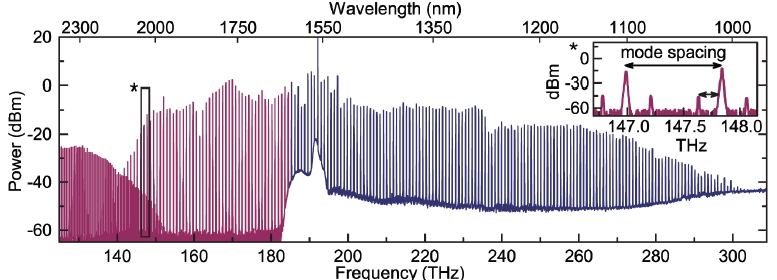
\includegraphics[]{octave_comb_mlg}
  %\caption{Спектр октавной гребенки, полученной из тороидального резонатора из плавленого кварца диаметром $40$ мкм. Расстояние между линиями гребенки $850$ ГГц. Взято из \cite{DelHaye2011}}
  %\label{octave_comb_mlg}
%\end{figure}


%В работе \cite{Herr2012} экспериментально изучалась динамика генерации гребенок в двух различных резонаторах: $MgF_2$ (ширина резонанса $1$ МГц), и $Si_3N_4$ (200 МГц). Геометрии резонаторов изображены на рис. \ref{mgf2_si3N4_resonators}.

%\begin{figure}
%  \centering
%  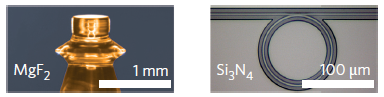
\includegraphics[]{mgf2_si3N4_resonators}
%  \caption{Форма резонаторов, в которых наблюдались оптические гребенки. Взято из \cite{Herr2012}}
%  \label{mgf2_si3N4_resonators}
%\end{figure}
%Для генерации первых боковых мод и далее всей гребенки лазер накачки постоянной мощности изначально сильно отстроен в синюю область от резонансной моды. Далее отстройка накачки медленно уменьшается, так что все больше и больше света связывается с резонансом. В некоторой точке достигается параметрический порог и возникает первая пара боковых мод. Экспериментальный вид спектра гребенок для обоих резонаторов представлен на рис. \ref{universal_formation_mlg}. Рассматриваются 2 сценария развития гребенки: а) первые образовавшиеся боковые моды являются соседними к моде накачки резонатора; б) первые боковые моды образуются вдалеке (по номеру моды) от накачки. Используется разложение собственных мод невозбужденного резонатора $\omega_\mu=\omega_0+D_1\mu+\frac{1}{2}D_2\mu^2$, где $D_1$ соответствует ОСД резонатора, $D_2$ - разность двух соседних ОСД около центральной частоты $\omega_0$. Далее аналитически решается система связанных уравнений для двух боковых мод и моды накачки. Собственные значения этой системы дают условие на порог генерации боковых мод. Откуда можно получить выражение для минимального номера первично возбуждаемых мод $\mu_{th,min}=\sqrt{\frac{\kappa}{D_2}}$, где $\kappa$ обозначает суммарные потери в резонаторе и элементе связи.
%\begin{figure}
%  \centering
%  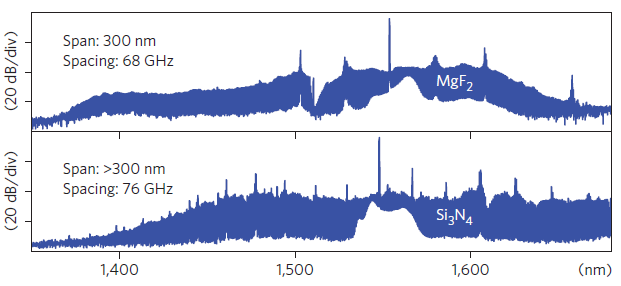
\includegraphics[]{universal_formation_mlg}
%  \caption{Спектр наблюдаемых гребенок. Мощность накачки для $MgF_2$ - $500$ мВт; для $Si_3N_4$ - $3$ Вт. Взято из \cite{Herr2012}}
%  \label{universal_formation_mlg}
%\end{figure}

%В работе \cite{Chembo2010pra} приводится общее описание сферических микрорезонаторов с модами типа шепчущей галереи (МШГ), дается вывод системы связанных уравнений (спектральное представление), описывающих динамику каждой моды. Аналитически выводится значение пороговой мощности, необходимой для начала генерации гребенки $P_{th}=\frac{n_0^2 V_0}{2\hbar\omega_0 n_2 c Q_0}$, где $n_0$ - показатель преломления, $V_0$ - эффективный объем моды, $\omega_0$ - частота накачки, $Q_0$ - собственная добротность резонатора, $n_2$ - нелинейная часть показателя преломления. В статье проведено численное моделирование этой системы для $200$ мод.

%Оптические гребенки наблюдались при разных геометриях резонаторов и разных типах связи с ними. В работе \cite{DelHaye2013} из цилиндрической заготовки из кварца при ее вращении выжигались $CO_2$ лазером резонаторы в форме микрокольца вокруг цилиндра диаметром от $170$ мкм до $8$ мм. В этих резонаторах удалось генерировать гребенку с расстоянием между модами от $300$ ГГц до $8.4$ ГГц соответственно. В работе \cite{Wang2013oe} использовался планарный кольцевой резонатор из нитрида кремния с использованием второго волновода для выходящего сигнала, при этом спектр на выходе был более гладким, т.к. спектральная линия большой мощности накачки не попадала в дроп-порт.

%Другой подход к моделированию оптических частотных гребенок основан не на системе связанных уравнений в спектральном представлении, а на решении уравнения Луджиато-Лефевера в пространственно-временном представлении. В работах \cite{Matsko2011} и \cite{Chembo2013} дан вывод этого уравнения из уравнений связанных мод. Решение уравнения Луджиато-Лефевера описывает в данном случае диссипативный временной солитон, распространяющийся в резонаторе. Экспериментальное наблюдение солитонов впервые было продемонстрировано в статье \cite{Herr2014}. Длительность солитона (полная ширина на половине высоты) составила около $200$ фс, период их следования около $28$ пс (для односолитонного режима). Экспериментальные данные первой демонстрации солитонов представлены на рис. \ref{experiment}

%\begin{figure}
%  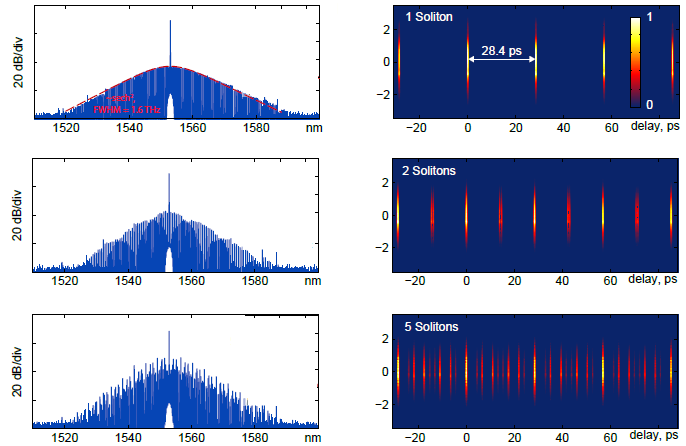
\includegraphics[]{experiment}
%  \caption{Экспериментально полученный спектр гребенки для одно-, двух и пяти солитонного режимов. Справа картина соответствующих импульсов во временном представлении. Взято из \cite{Herr2014}} \label{experiment}
%\end{figure}

%Обзор потенциальных применений оптических гребенок в микрорезонаторах дан в \cite{Kippenberg2011}. Используя компактные микрорезонаторы и один лазер накачки, можно сделать калибровку для астрономического спектрографа для видимого и ближнего ИК диапазонов, с межмодовым расстоянием $10-30$ ГГц. Такие устройства могут позволить измерить доплеровский сдвиг в спектре звезды с точностью, требуемой для обнаружения планет вне Солнечной системы. Ключевым преимуществом в этом случае является малый размер и масса системы.
